
\documentclass[tikz]{standalone}
\begin{document}
% Kante %
\begin{tikzpicture}
    \draw (0,0) -- (1, .5);
\end{tikzpicture}
% Kreis %
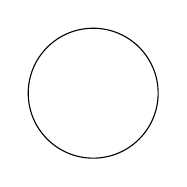
\begin{tikzpicture}
    \draw (0,0) circle (.825);
\end{tikzpicture}
% Node %
\tikzstyle{MeinKreis} = [circle]
\tikzstyle{MeineKante} = [line]
\begin{tikzpicture}
    \node (K1) at (0,0) [MeinKreis] {a};
    \node (K2) at (4,1) [MeinKreis] {b};
    \draw [MeineKante] (K1) -- (K2);
\end{tikzpicture}


\end{document}